В экспериментах мы сравниваем три различных постановки: алгоритм SimCLR как self-supervised learning метод, обучение с учителем на примере классификации изображений и обучение со случайной разметкой по классам. В качестве случайной разметки используется фиксированная случайная перестановка классов обучающих объектов, что позволяет сохранить исходный баланс классов. Эксперименты проводятся на наборе данных CIFAR-10 \cite{cifar}, используется архитектура сверточной нейронной сети ResNet-18 \cite{resnet}. Аугментации изображений играют значимую роль в первых двух постановках, поэтому обучение со случайной разметкой мы рассматриваем в двух вариациях: с использованием аугментаций и без них. При этом в алгоритме SimCLR применяются более интенсивные аугментации, чем при обучении с учителем. При обучении со случайной разметкой используются те же аугментации, что и при обучении с учителем. Более подробное описание типов аугментаций, а также других гиперпараметров обучения доступно в \hyperref[appendix:1]{Приложении А}.

Наши эксперименты устанавливают, как меняются предсказания нейронных сетей по ходу обучения. Кроме того, мы проверяем, что обуславливает сложность выучивания тех или иных объектов. Мы устанавливаем, что сами объекты обладают неодинаковой сложностью в контексте рассмотренных постановок обучения. Вдобавок мы изучаем влияние аугментаций на сложность объектов и показываем, что аугментации в методе SimCLR увеличивают разброс сложности объектов (то есть выделяются очень простые и очень сложные изображения), в то время как сложности, ассоциированные с самими объектами, являются более однородными.

\subsection{Динамика обучения}

Наш подход к изучению динамики обучения вдохновлен \cite{memorization}. В \hyperref[simclr:1]{разделе 3} показано, что алгоритм SimCLR эквивалентен задаче классификации внутри пакета размера $B$ с $2B-1$ классом. Таким образом, все упомянутые постановки представляют собой задачи классификации. Рассмотрим нейронную сеть $f_{\theta}: \R^{H \times W \times C} \rightarrow [0, 1]^L$, параметризованную весами $\theta \in \R^{\Theta}$, которая предсказывает вероятности $L$ классов. Пусть вероятность класса $y \in \{1, \dots, L\}$ для изображения $x \in \R^{H \times W \times C}$ обозначается как $p_{\theta}(y|x)$, $\sum_{y=1}^L p_{\theta}(y|x)=1$. Пусть также $y_{\text{true}}$ --- истинный класс изображения $x$. Тогда событие $y_{\text{true}} = \argmax_{y} p_{\theta}(y|x)$ означает, верно ли изображение $x$ классифицировано нейронной сетью $f_{\theta}$.

Рассмотрим теперь $\theta \sim \mathcal{T}(t)$ --- распределение весов нейронной сети $f_{\theta}$ после $t$ эпох обучения (здесь в случайность входит начальная инициализация, перемешивание объектов стохастического градиентного спуска и аугментации изображений обучающей выборки). Напомним также, что $\mathcal{A}(\tilde{x}|x)$ обозначает распределение аугментаций изображения $x$. Центральной величиной является $r_t(x)$ --- вероятность того, что аугментированное изображение $x$ правильно классифицируется после $t$ эпох обучения:
\begin{equation}
    r_t(x) = \mathbb{P}_{\substack{\theta \sim \mathcal{T}(t) \\ \tilde{x} \sim \mathcal{A}(\tilde{x}|x)}} \Big(y_{\text{true}} = \argmax_{y} p_{\theta}(y|\tilde{x})\Big)
\end{equation}

Мы переписываем вероятность события как мат. ожидание индикатора и оцениваем его методом Монте-Карло, обучая несколько копий нейронной сети из разных начальных инициализаций:
\begin{equation}
\label{experiments:eq:1}
\begin{gathered}
    r_t(x) = \E_{\substack{\theta \sim \mathcal{T}(t) \\ \tilde{x} \sim \mathcal{A}(\tilde{x}|x)}} \Big[\big[y_{\text{true}} = \argmax_{y} p_{\theta}(y|\tilde{x})\big]\Big] \approx \\
    \approx \frac{1}{NM} \sum_{i=1}^N\sum_{j=1}^M \big[y_{\text{true}} = \argmax_{y} p_{\theta_i}(y|\tilde{x}_j)\big],
\end{gathered}
\end{equation}

\noindent
где $N$ --- число копий нейронной сети, $\theta_i \sim \mathcal{T}(t)$ --- веса одной копии, \linebreak $M$ --- число аугментаций, $\tilde{x}_j \sim \mathcal{A}(\tilde{x}|x)$ --- одна аугментация изображения. В экспериментах используются значения $N=30, M=10$.

Мы анализируем динамику обучения различных постановок, оценивая величину $r_t(x)$ на некоторой фиксированной подвыборке обучающих объектов. При этом для каждого алгоритма используется то же самое распределение аугментаций, что и при обучении (в частности, при обучении со случайной разметкой аугментации не используются, а значит, распределение аугментаций в этом случае вырождается в дельта-распределение в точке исходного изображения: $\mathcal{A}(\tilde{x}|x) = \delta(\tilde{x} - x)$).

\begin{figure}[H]
    \centering
    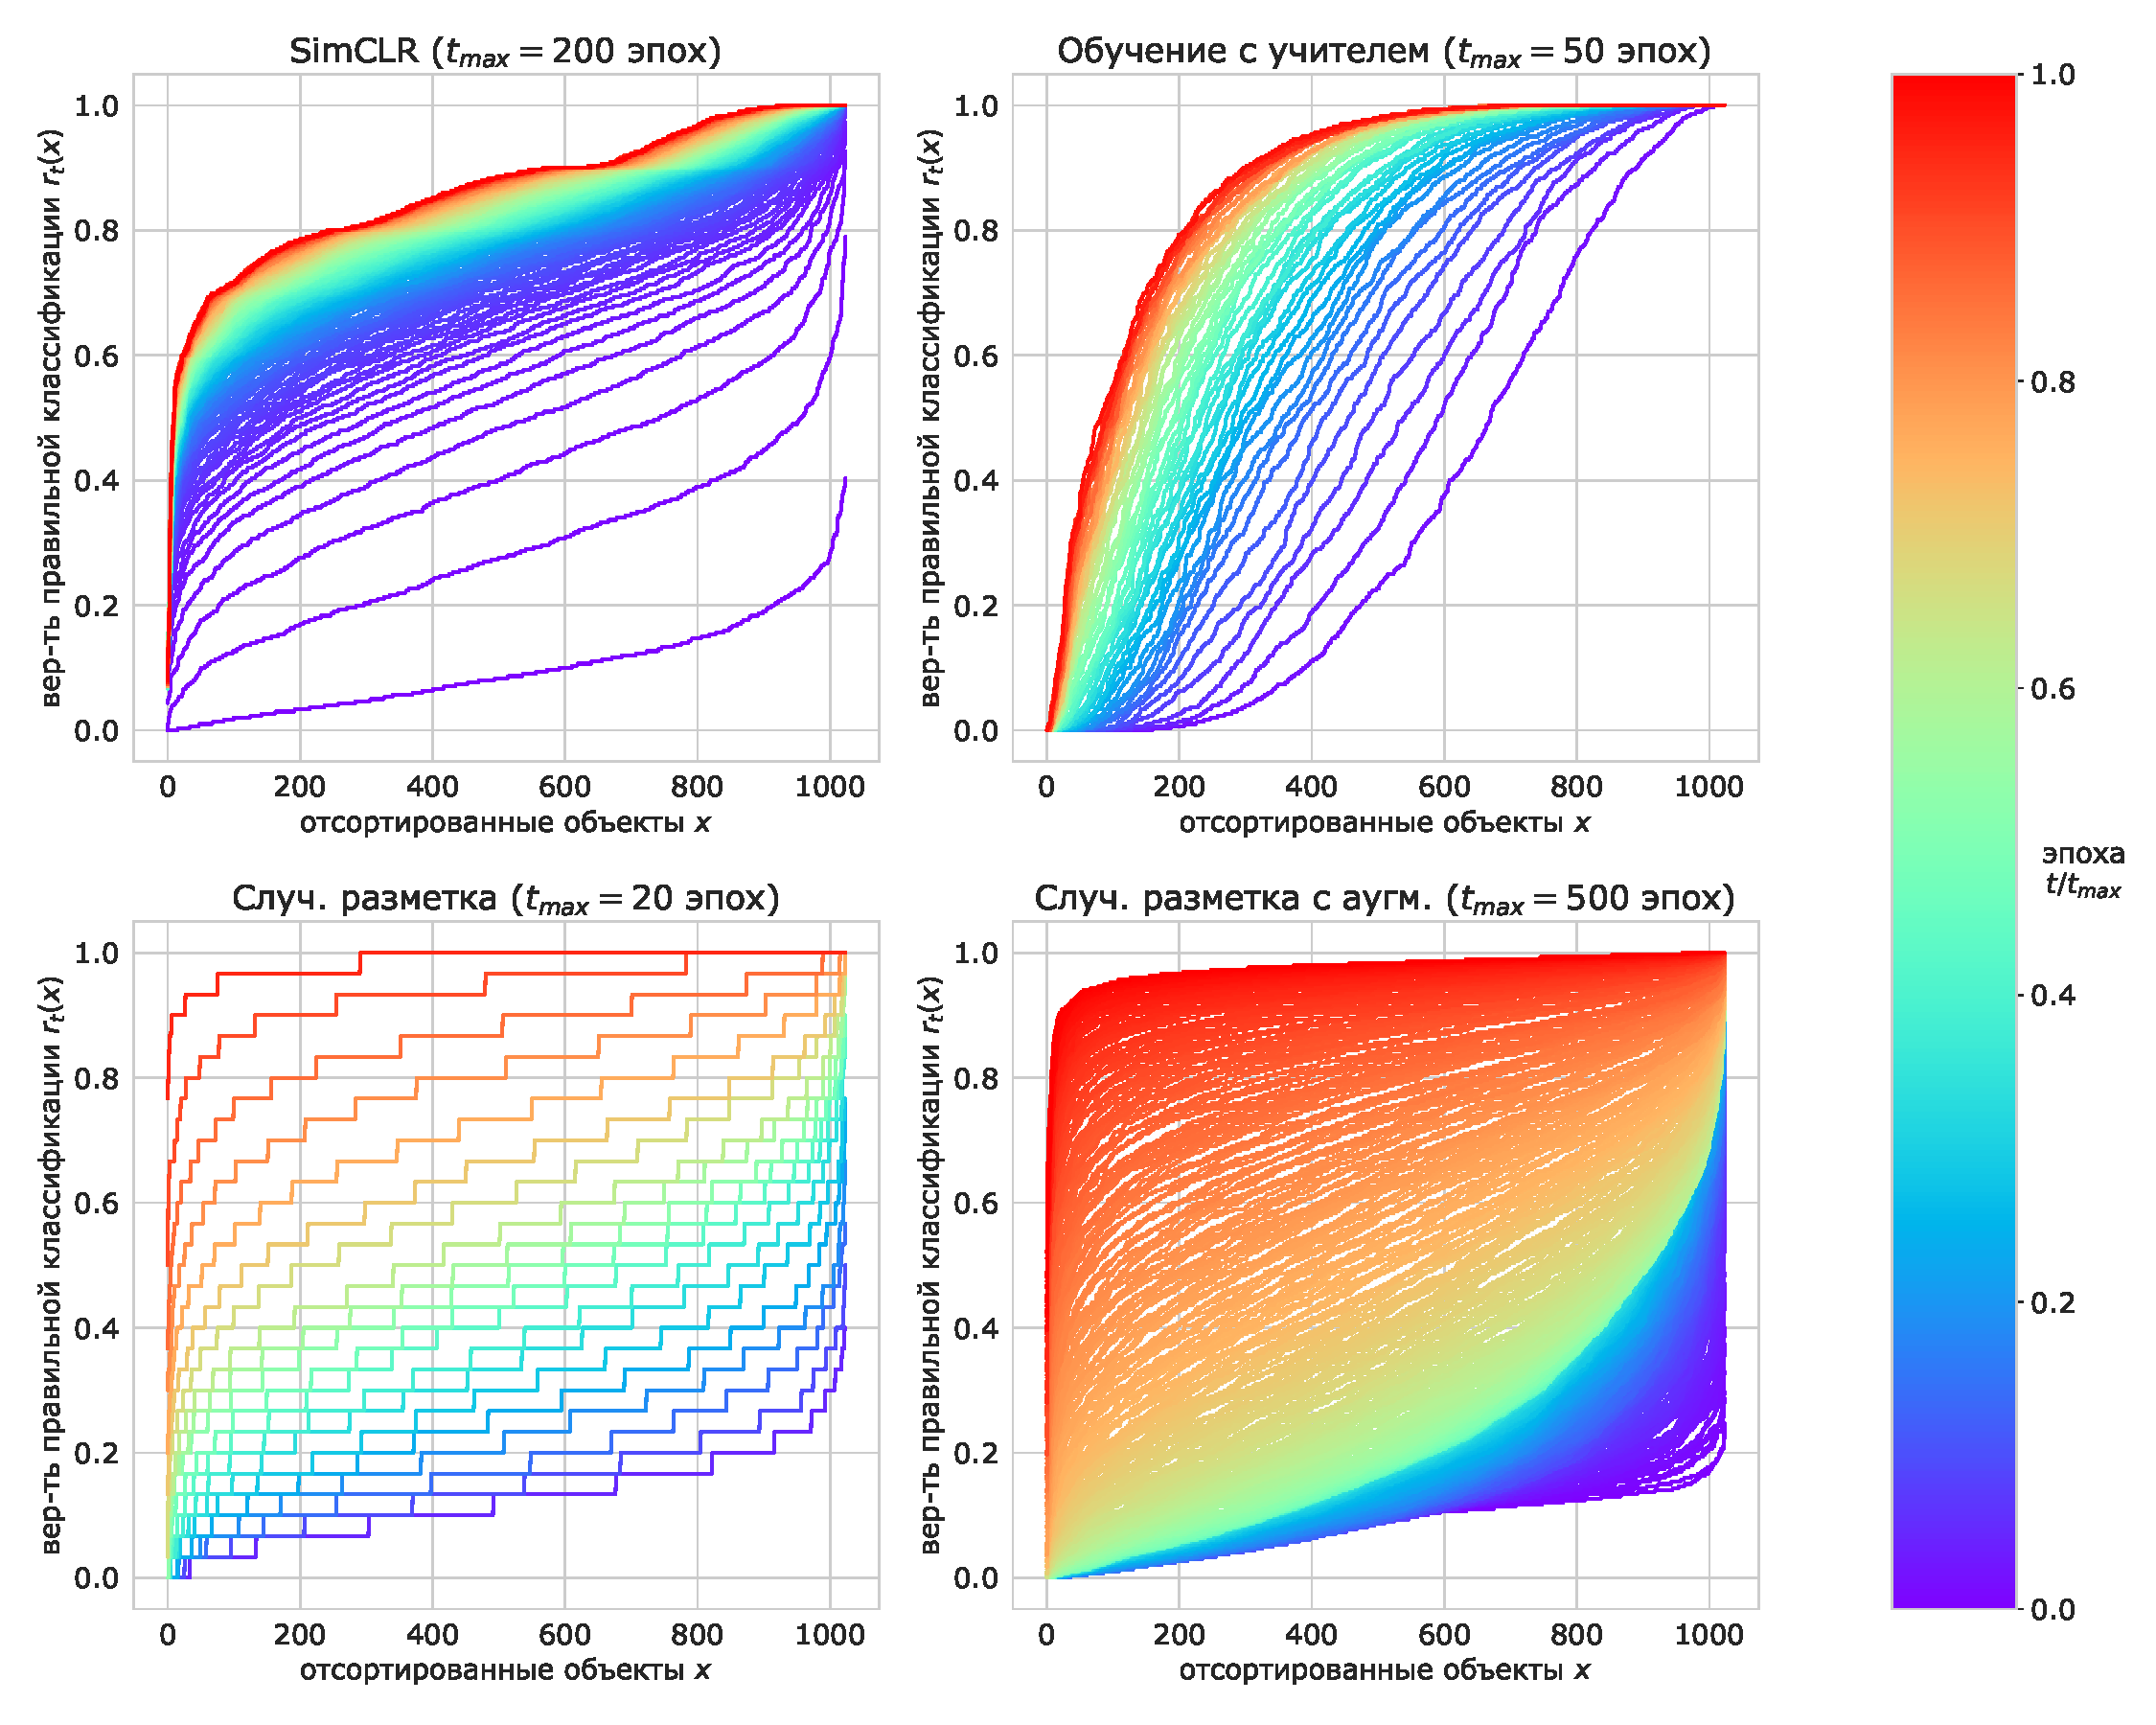
\includegraphics[width=17cm]{images/training_dynamics.pdf}
    \caption{Динамика обучения различных методов. По горизонтальной оси отложены объекты из обучающей подвыборки размера $K=1024$, отсортированные по величине $r_t(x)$ независимо по эпохам, по вертикальной оси - показатель $r_t(x)$. Цвет линии для каждой эпохи $t$ выставлен относительно максимального числа эпох $t_{\max}$ (своё для каждого метода). Ввиду отсутствия усреднения по аугментациям рисунок для обучения со случайной разметкой имеет характерный ступенчатый вид с высотой ступеней 1/N.}
    \label{experiments:pic:1}
\end{figure}{}

Также стоит отметить, что в методе SimCLR для каждого изображения $x$ есть по две отдельные задачи классификации, так как используются две его аугментации $\tilde{x}_1, \tilde{x}_2 \sim \mathcal{A}(\tilde{x}|x)$. Соответственно, для аугментации $\tilde{x}_1$ правильным классом является $\tilde{x}_2$, и наоборот. Условные вероятности $p_{\theta}(\tilde{x}_2|\tilde{x}_1)$ и $p_{\theta}(\tilde{x}_1|\tilde{x}_2)$, вообще говоря, не равны. Индикаторы для $\tilde{x}_1$ и $\tilde{x}_2$ из ур. \ref{experiments:eq:1} также могут отличаться, отчего не ясно, какой именно индикатор подставлять в формулу $r_t(x)$. Однако наличие усреднения по аугментациям решает данную проблему (не имеет значения, какой из двух индикаторов использовать), что подтверждается дополнительными материалами, изложенными в \hyperref[appendix:2]{Приложении Б}.

На рис. \ref{experiments:pic:1} показана эволюция величины $r_t(x)$ различных методов от начальных и до финальных эпох обучения. Кривая для каждой эпохи представляет собой отсортированные значения $r_t(x)$. Однако рассмотренные методы имеют разную скорость обучения, поэтому максимальное число эпох $t_{\max}$ своё у каждого метода. Данный график демонстрирует, что методы имеют непохожее распределение $r_t(x)$, особенно выделяются кривые обучения с учителем, имеющие s-образную форму на ранних стадиях обучения. Дальнейший анализ направлен на более подробное сравнение методов.

Как уже обсуждалось выше, методы имеют разную скорость обучения, поэтому для справедливого сравнения их необходимо уравнять по эпохам. Пусть $\mathcal{D}$ --- это распределение изображений обучающей выборки. Мы предлагаем сопоставлять эпохи обучения друг другу по величине $\E_{x \sim \mathcal{D}} \big[r_t(x)\big]$ --- средней по обучающим объектам вероятности правильной классификации. Данную величину мы также оцениваем методом Монте-Карло по обучающей подвыборке размера $K=1024$:
\begin{equation}
    \E_{x \sim \mathcal{D}} \big[r_t(x)\big] \approx \frac{1}{K} \sum_{k=1}^K r_t(x_k)
\end{equation}

\noindent
Данная оценка приближенно совпадает с площадью под отсортированной кривой $r_t(x)$, как на рис. \ref{experiments:pic:1}. Из графика следует, что площадь под кривой растет по ходу обучения, поэтому уравнивать алгоритмы по указанному показателю представляется разумным.

Далее, рассмотрим два алгоритма обучения $A$ и $B$. Зафиксируем число эпох обучения алгоритма A как $t_A$. Тогда соответствующее ему число эпох $t_B$ алгоритма $B$ определяется как:
\begin{equation}
    t_B = \argmin_t \Big|\E_{x \sim \mathcal{D}} \big[r^A_{t_A}(x)\big] - \E_{x \sim \mathcal{D}} \big[r^B_{t}(x)\big]\Big|,
\end{equation}

\noindent
где величина $r^A_{t}(x)$ относится к алгоритму $A$, а $r^B_{t}(x)$ --- к алгоритму $B$. Поскольку данные для оценки $r_t(x)$ собираются в дискретные моменты времени обучения (раз в эпоху), то достичь точного равенства мат. ожиданий не удается, но описанная эвристика позволяет сопоставить стадии обучения различных методов.

\begin{figure}[H]
    \centering
    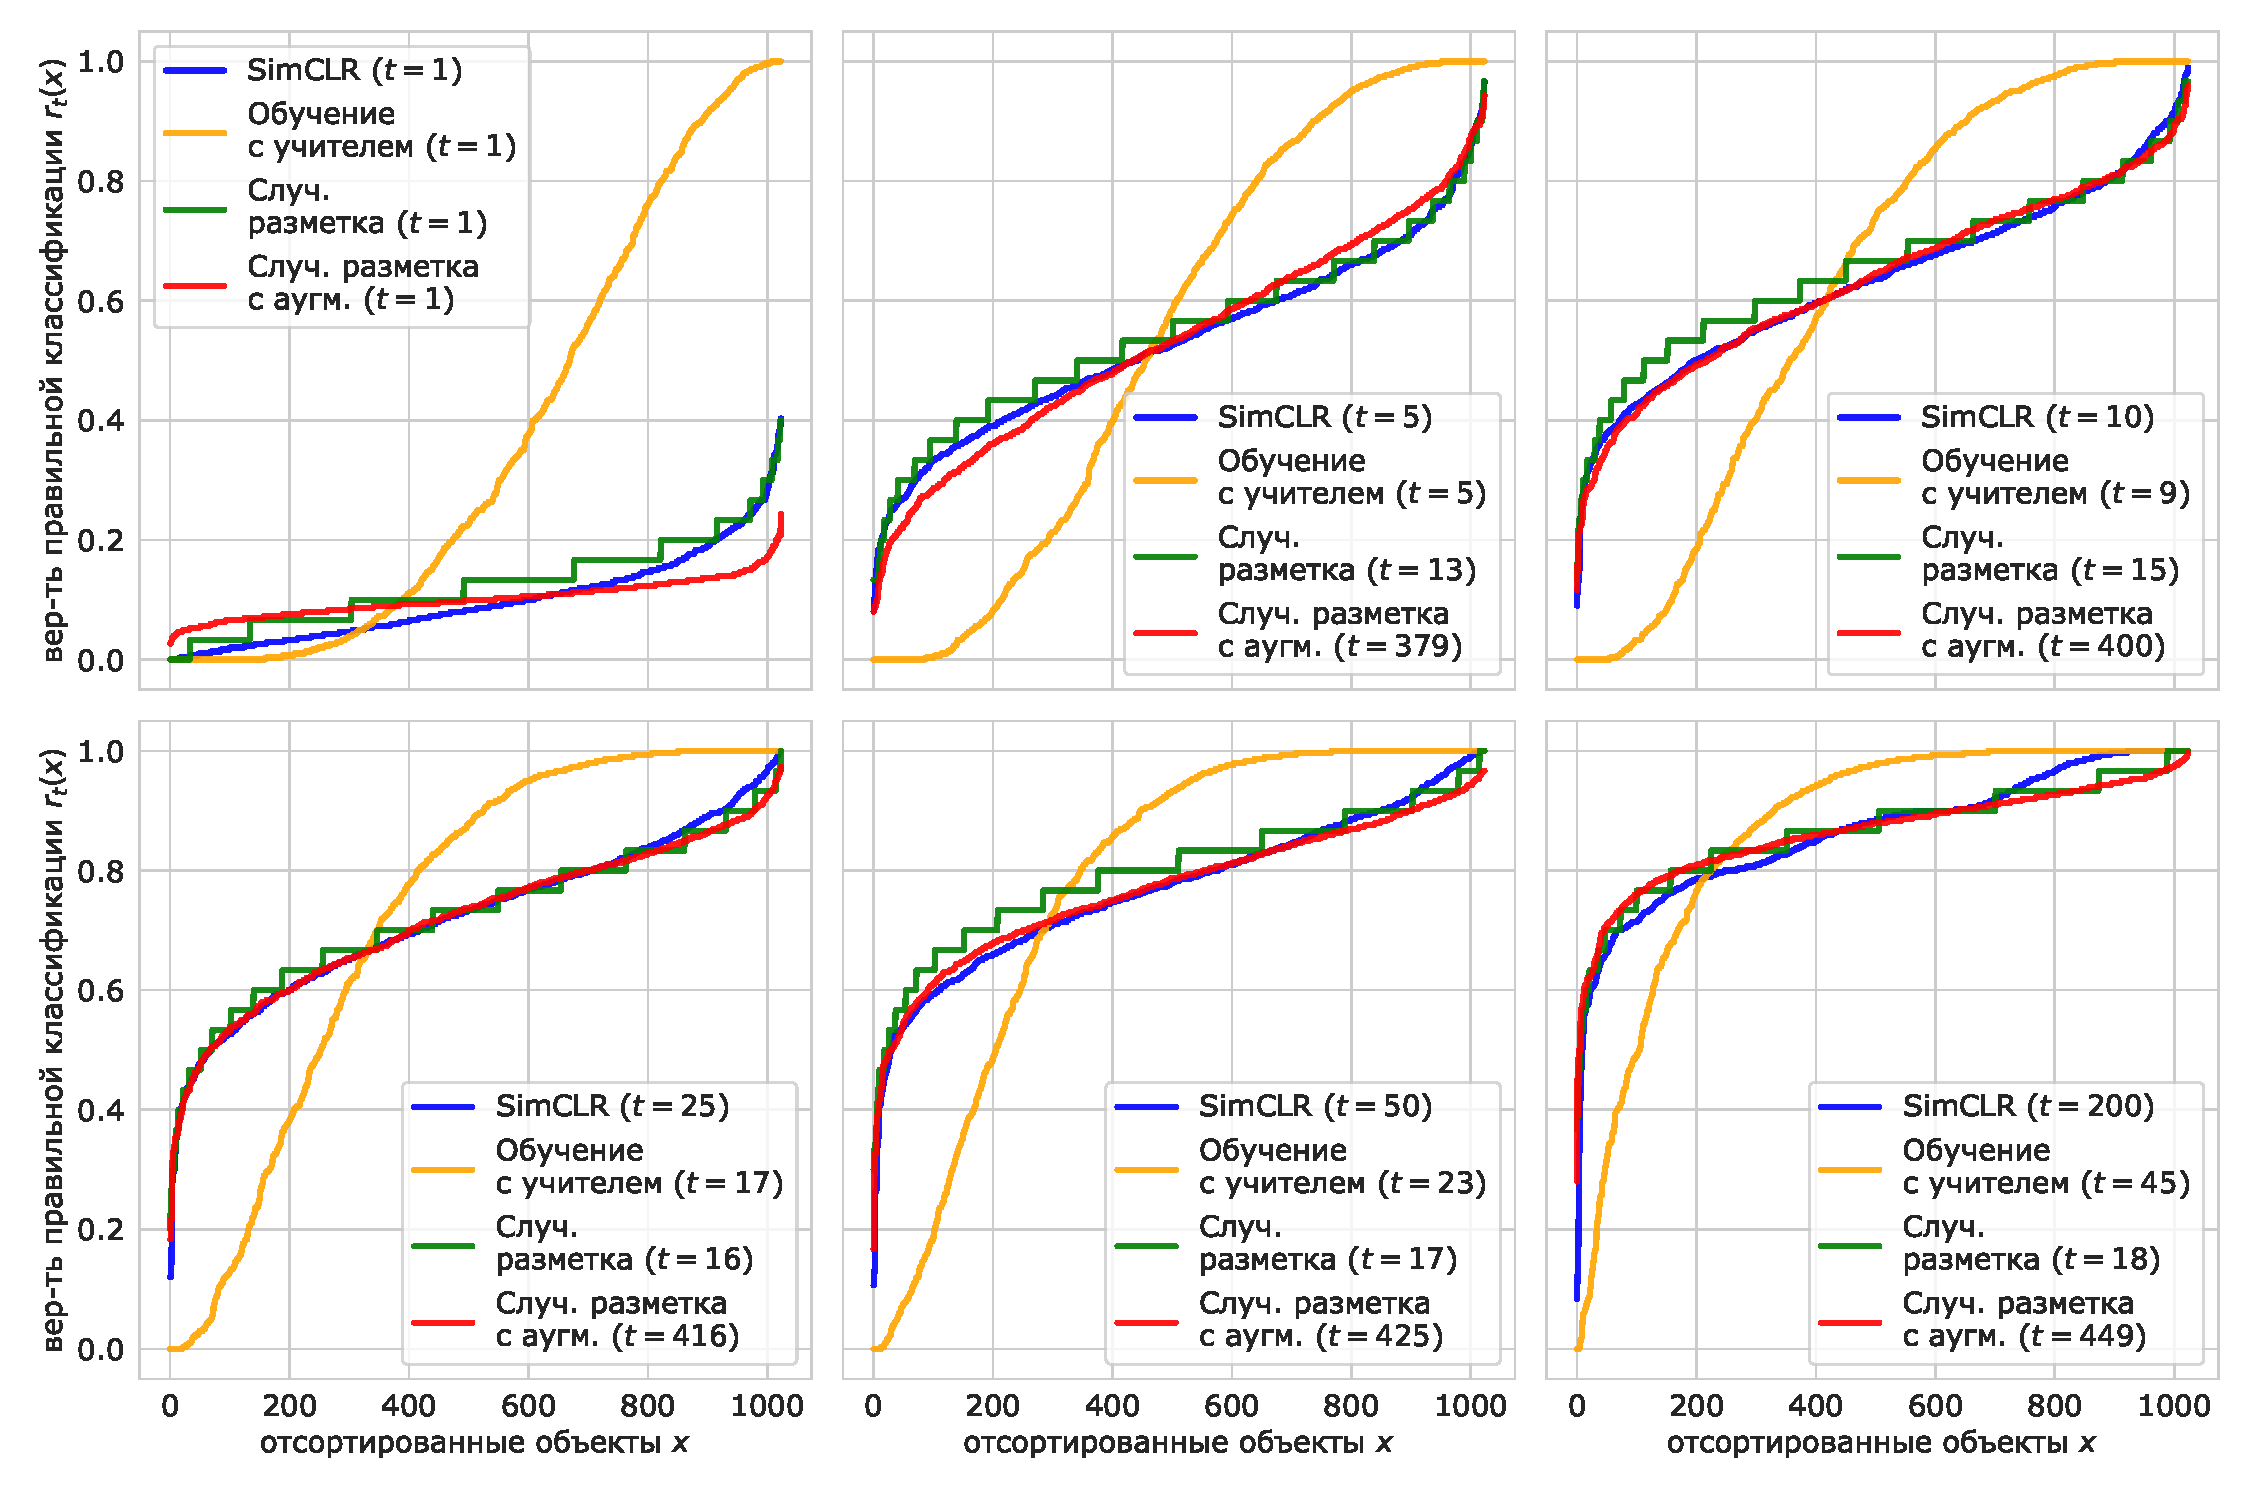
\includegraphics[width=17cm]{images/equal_areas.pdf}
    \caption{Сравнение динамики обучения методов. Обозначения в скобках показывают число эпох $t$ обучения при подсчете величины $r_t(x)$.}
    \label{experiments:pic:2}
\end{figure}{}

На рис. \ref{experiments:pic:2} представлен результат сравнения динамики обучения алгоритмов с учетом выравнивания по эпохам. Опорным методом для сопоставления эпох выбран SimCLR, рассмотрены значения $t \in \{1, 5, 10, 25, 50, 200\}$. Неожиданным выводом здесь оказывается, что динамика обучения метода SimCLR очень похожа на динамику обучения со случайной разметкой. Мы предлагаем следующую интуицию, объясняющую данный феномен: в обеих постановках нейронная сеть должна научиться непосредственно распознавать изображения обучающей выборки. В случае метода SimCLR каждое изображение, по сути, является отдельным классом, а аугментации изображения - примерами класса. При обучении со случайной разметкой последняя не несет никакой информации об объектах, так что для правильной классификации обучающей выборки от нейронной сети требуется запомнить все обучающие примеры. При обучении с учителем, напротив, разметка является информативной, и нейронной сети достаточно выделить фрагменты изображений, специфичные для каждого класса, отчего нет необходимости заучивать обучающую выборку, что и приводит к другой форме кривой $r_t(x)$.

\subsection{Сравнение с биномиальным шумом}
\label{experiments:1}

Следующая серия экспериментов проверяет гипотезу о простых и сложных объектах, сформулированную в \cite{memorization}: нейронные сети выучивают некоторые объекты обучающей выборки быстрее, чем остальные. Предположим, что гипотеза не верна, и все обучающие объекты $x$ имеют одинаковую сложность. Тогда случайная величина $[y_{\text{true}} = \argmax_{y} p_{\theta}(y|x)]$ зависит от распределения $\theta \sim \mathcal{T}(t)$, но не от $x \sim \mathcal{D}$. Поскольку индикатор принимает бинарные значения, то можно считать, что он имеет распределение Бернулли с некоторой вероятностью $p_0$, не зависящей от объекта $x$. Индикатор зависит только от $\theta$, поэтому при независимых $\theta_1, \theta_2 \sim \mathcal{T}(t)$ соответствующие им индикаторы также будут независимыми.

Теперь для каждого изображения $x$ зафиксируем его случайную аугментацию $\tilde{x} \sim \mathcal{A}(\tilde{x}|x)$ и рассмотрим величину $\tilde{r}_t(\tilde{x})$:
\begin{equation}
\begin{gathered}
    \tilde{r}_t(\tilde{x}) = \mathbb{P}_{\theta \sim \mathcal{T}(\theta)} \Big(y_{\text{true}} = \argmax_{y} p_{\theta}(y|\tilde{x})\Big) = \\
    = \E_{\theta \sim \mathcal{T}(t)} \Big[\big[y_{\text{true}} = \argmax_{y} p_{\theta}(y|\tilde{x})\big]\Big] \approx \frac{1}{N} \sum_{i=1}^N [y_{\text{true}} = \argmax_{y} p_{\theta_i}(y|\tilde{x})]
\end{gathered}
\end{equation}

\noindent
Фактически, $\tilde{r}_t(\tilde{x})$ отличается от рассмотренной выше $r_t(x)$ отсутствием \linebreak усреднения по аугментациям. Итак, если все аугментированные изображения имеют одинаковую сложность, то случайная величина $\tilde{r}_t(\tilde{x})$ распределена биномиально с точностью до константы $1/N$ (как сумма независимых бернуллиевских случайных величин):
\begin{equation}
\begin{gathered}
    \tilde{r}_t(\tilde{x}) \approx \frac{1}{N} \sum_{i=1}^N [y_{\text{true}} = \argmax_{y} p_{\theta_i}(y|\tilde{x})] \sim \frac{1}{N} \sum_{i=1}^N \text{Bern}(p_0) = \\
    = \frac{1}{N} \text{Bin}(N, p_0)
\end{gathered}
\end{equation}

Далее, для каждого метода обучения мы предлагаем проверить нулевую гипотезу, что случайная величина $N \tilde{r}_t(\tilde{x})$ имеет биномиальное распределение $\text{Bin}(N, \widehat{p}_0(t))$. Для этого мы оцениваем параметр $\widehat{p}_0(t)$ по выборке:
\begin{equation}
    \widehat{p}_0(t) = \frac{1}{K} \sum_{k=1}^K \tilde{r}_t (\tilde{x}_k) 
\end{equation}

\noindent
Для проверки гипотезы используется хи-квадрат тест равенства частот \cite{chisquare}. При этом число степеней свободы распределения хи-квадрат уменьшается на 1 за счет оценивания по данным одного параметра $\widehat{p}_0(t)$.

Чтобы не проводить тестирование гипотезы для каждой эпохи обучения, мы выделяем по 3 эпохи на каждый алгоритм. Для $p_0 \in [0.25, 0.5, 0.75]$ мы выбираем первую по порядку эпоху $t$, при которой $\widehat{p}_0(t) > p_0$. Таким образом, всего проверяется 12 гипотез --- для каждой из 3 эпох по 4 алгоритмам.

\begin{figure}[H]
    \centering
    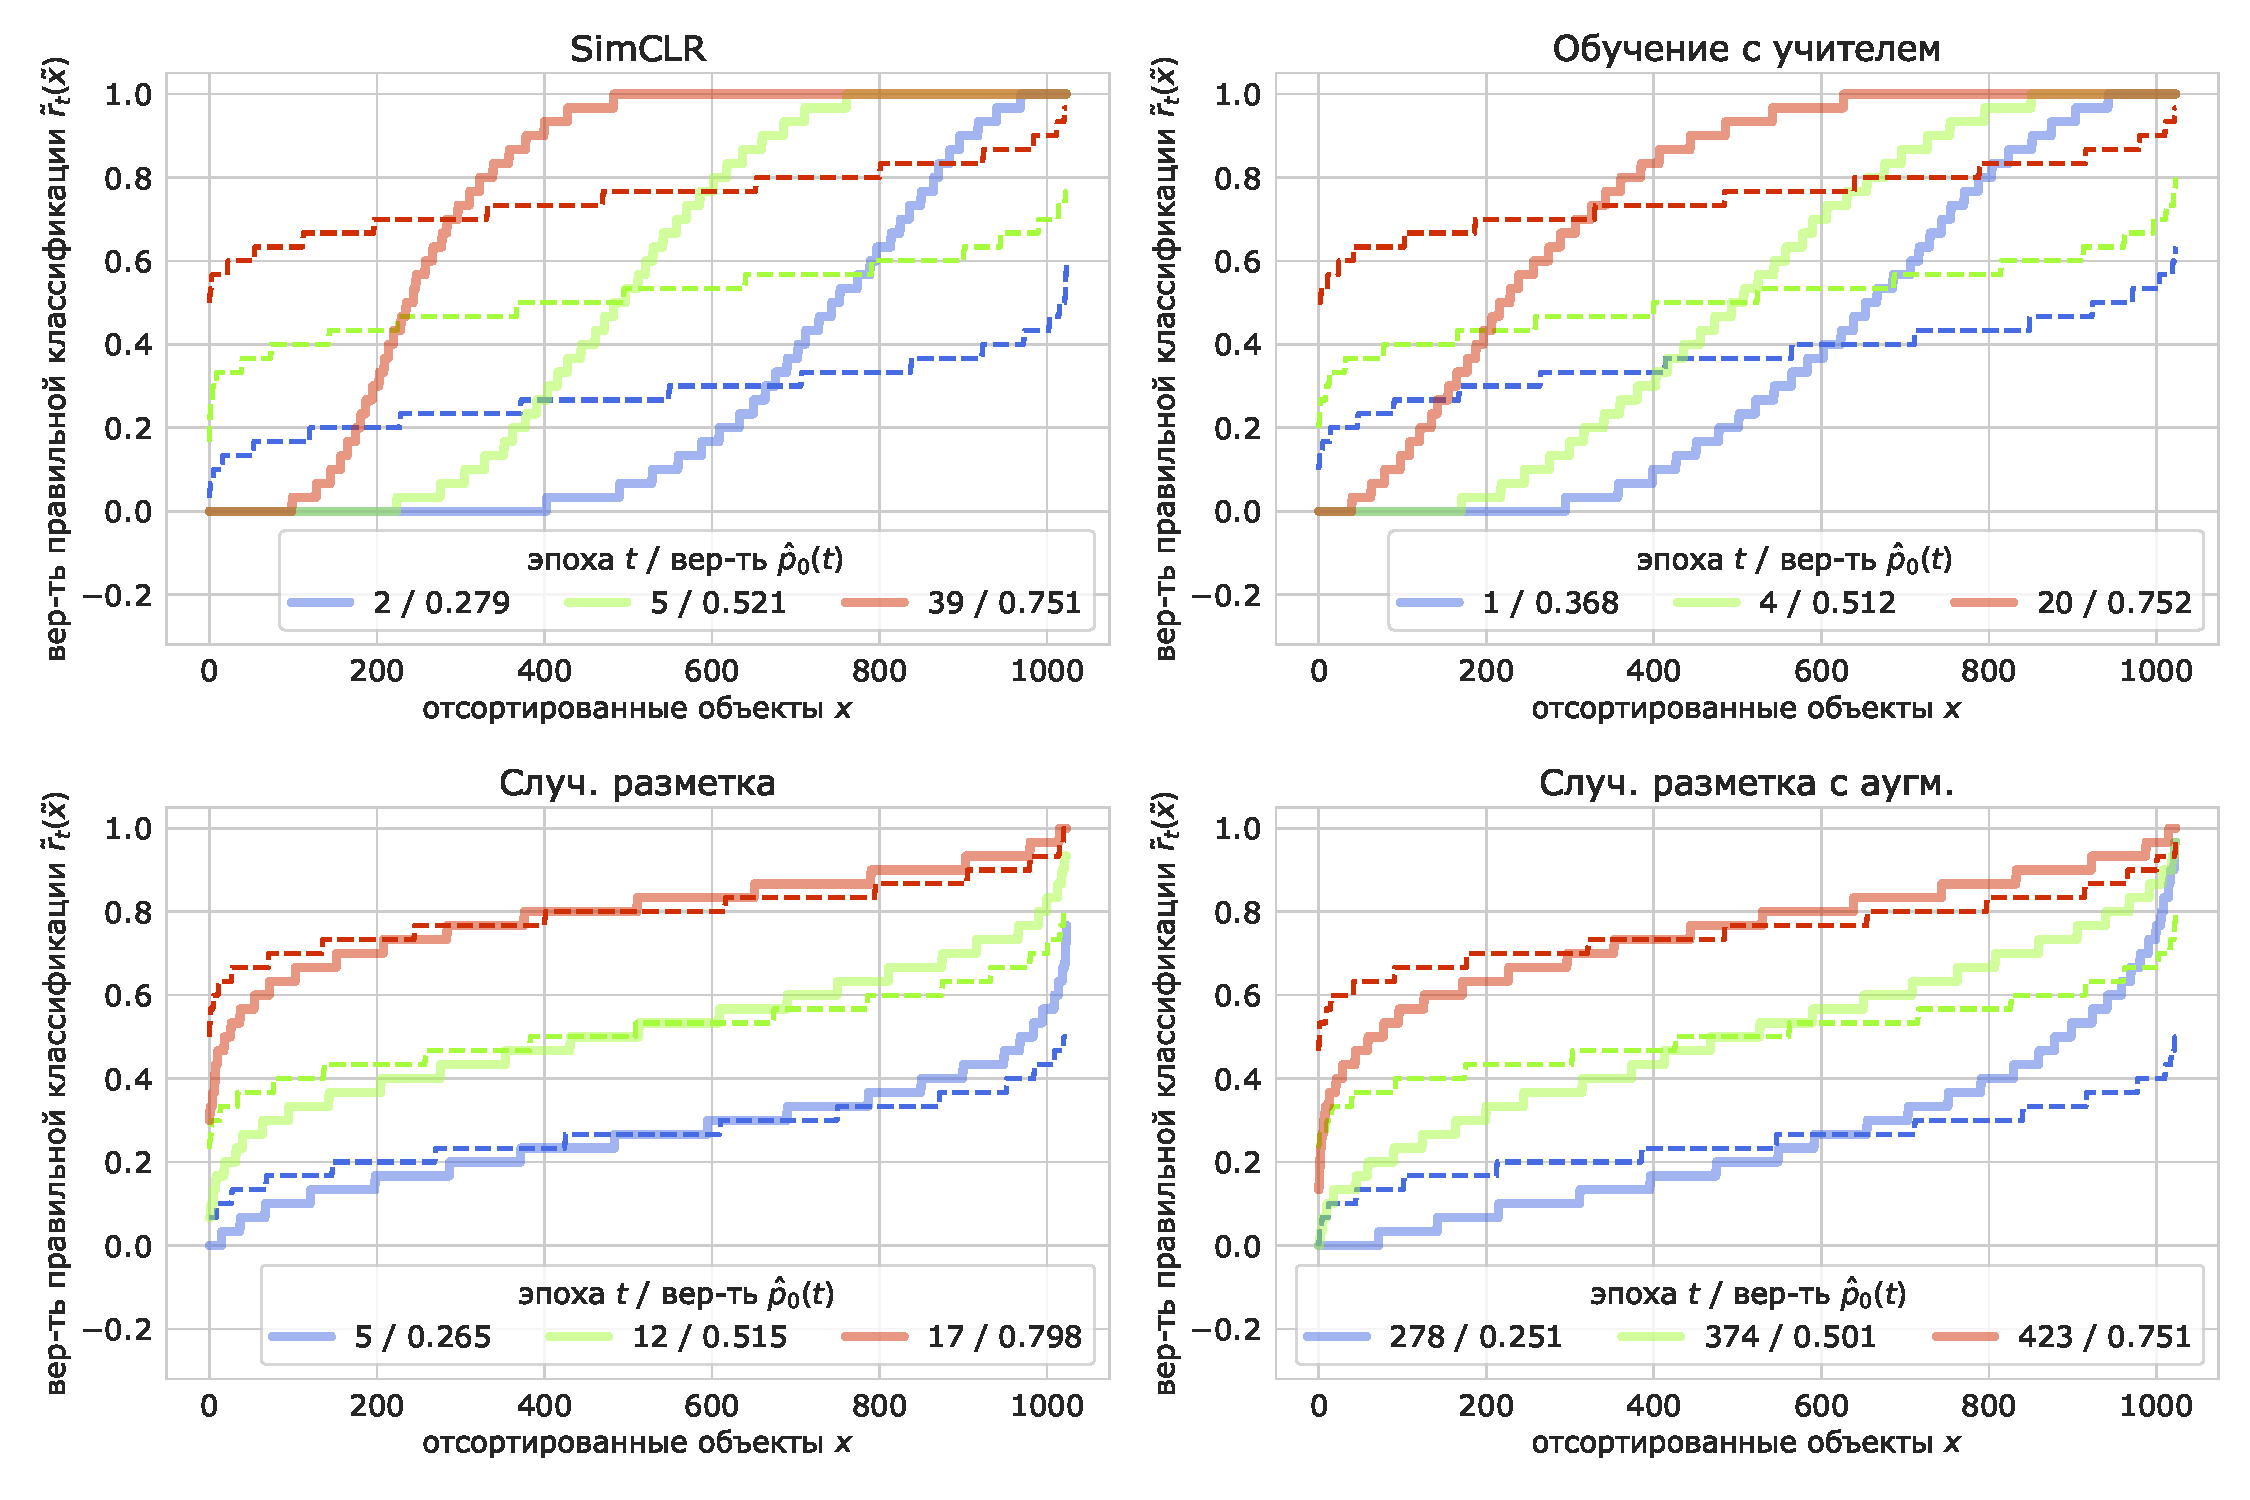
\includegraphics[width=17cm]{images/binom_noise1.pdf}
    \caption{Сравнение величины $\tilde{r}_t(\tilde{x})$ (сплошная жирная линия) с соответствующим биномиальным шумом (пунктирная линия).}
    \label{experiments:pic:3}
\end{figure}{}

Из рис. \ref{experiments:pic:3} становится очевидно, что нулевая гипотеза не верна. Это же подтверждается и результатами теста, приведенными в таблице \ref{experiments:table:1}. Таким образом, аугментированные изображения имеют разную сложность в контексте всех четырех алгоритмов. Тем не менее, нельзя не отметить, что распределение $\tilde{r}_t(\tilde{x})$ обучения со случайной разметкой больше всего напоминает биномиальное: это заметно и по графикам, и по меньшим значениям тестовой статистики $\chi^2$. Данное наблюдение свидетельствует о том, что при обучении со случайной разметкой объекты имеют меньший разброс сложности. Напротив, при отсутствии усреднения по аугментациям кривые метода SimCLR становятся похожи на кривые обучения с учителем. Данные кривые сильно отличаются от биномиального шума, то есть присутствуют как очень простые, так и очень сложные объекты. Мы предполагаем, что конкретные аугментации увеличивают разброс сложности объектов, и потому проводим похожий эксперимент с добавлением усреднения по аугментациям.

\begin{table}[H]
    \centering
    \begin{tabular}{|C{2.5cm}|C{1.75cm}|C{2.75cm}|C{3.25cm}|C{2.75cm}|}
        \hline
        Метод & Эпоха $t$ & Вер-ть $\widehat{p}_0(t)$ & Тест. статистика $\chi^2$ & P-значение \\ \hline
        \multirow{3}{*}{SimCLR} & 2 & 0.279 & $1.3 \cdot 10^{17}$ & 0.0 \\ \cline{2-5}
        & 5 & 0.521 & $2.1 \cdot 10^{11}$ & 0.0 \\ \cline{2-5}
        & 39 & 0.751 & $1.3 \cdot 10^{19}$ & 0.0 \\ \hline
        \multirow{3}{*}{\shortstack{Обучение\\с учителем}} & 1 & 0.368 & $6.7 \cdot 10^{13}$ & 0.0 \\ \cline{2-5}
        & 4 & 0.512 & $8 \cdot 10^{10}$ & 0.0 \\ \cline{2-5}
        & 20 & 0.752 & $2.4 \cdot 10^{18}$ & 0.0 \\ \hline
        \multirow{3}{*}{\shortstack{Случ.\\разметка}} & 5 & 0.265 & $8.4 \cdot 10^{4}$ & 0.0 \\ \cline{2-5}
        & 12 & 0.515 & $4.2 \cdot 10^{4}$ & 0.0 \\ \cline{2-5}
        & 17 & 0.798 & $4.5 \cdot 10^{5}$ & 0.0 \\ \hline
        \multirow{3}{*}{\shortstack{Случ.\\разметка\\с аугм.}} & 278 & 0.251 & $4.4 \cdot 10^{13}$ & 0.0 \\ \cline{2-5}
        & 374 & 0.501 & $5.2 \cdot 10^{6}$ & 0.0 \\ \cline{2-5}
        & 423 & 0.751 & $5.9 \cdot 10^{8}$ & 0.0 \\ \hline
    \end{tabular}
    \caption{Результаты хи-квадрат теста. Все нулевые гипотезы и так отклоняются, поэтому поправка на множественное тестирование гипотез не требуется.}
    \label{experiments:table:1}
\end{table}

Мы расширяем анализ на величину $r_t(x)$, чтобы исключить влияние аугментаций на сложность объектов. Усреднение по аугментациям заметно усложняет теоретический вывод. Ур. \ref{experiments:eq:1} можно переписать в следующем виде:
\begin{equation}
    r_t(x) \approx \frac{1}{N} \sum_{i=1}^N \bigg( \frac{1}{M} \sum_{j=1}^M \big[y_{\text{true}} = \argmax_{y} p_{\theta_i}(y|\tilde{x}_j)\big] \bigg)
\end{equation}

\noindent
Из-за наличия зависимостей между аугментациями одного изображения слагаемое в скобках уже нельзя представить в виде простого распределения (получается некоторое дискретное распределение на множестве $\{0, 1/M, \dots, 1\}$). Мы предлагаем провести менее формальный анализ, приняв биномиальное распределение за образец однородной сложности объектов. В качестве метрики мы используем среднюю абсолютную ошибку (англ. mean absolute error, MAE) между отсортированными кривыми $r_t(x)$ (приблизительно равна площади между кривыми):
\begin{equation}
    \text{MAE}\Big(\{x_k\}_{k=1}^K, \{b_k\}_{k=1}^K\Big) = \frac{1}{K} \sum_{k=1}^K |r_t(x_k) - b_k|,
\end{equation}

\noindent
где значения $r_t(x_k)$ и $b_k$ отсортированы по возрастанию и $b_k \sim \text{Bin}(N, \widehat{p}_0(t))$.

\begin{figure}[H]
    \centering
    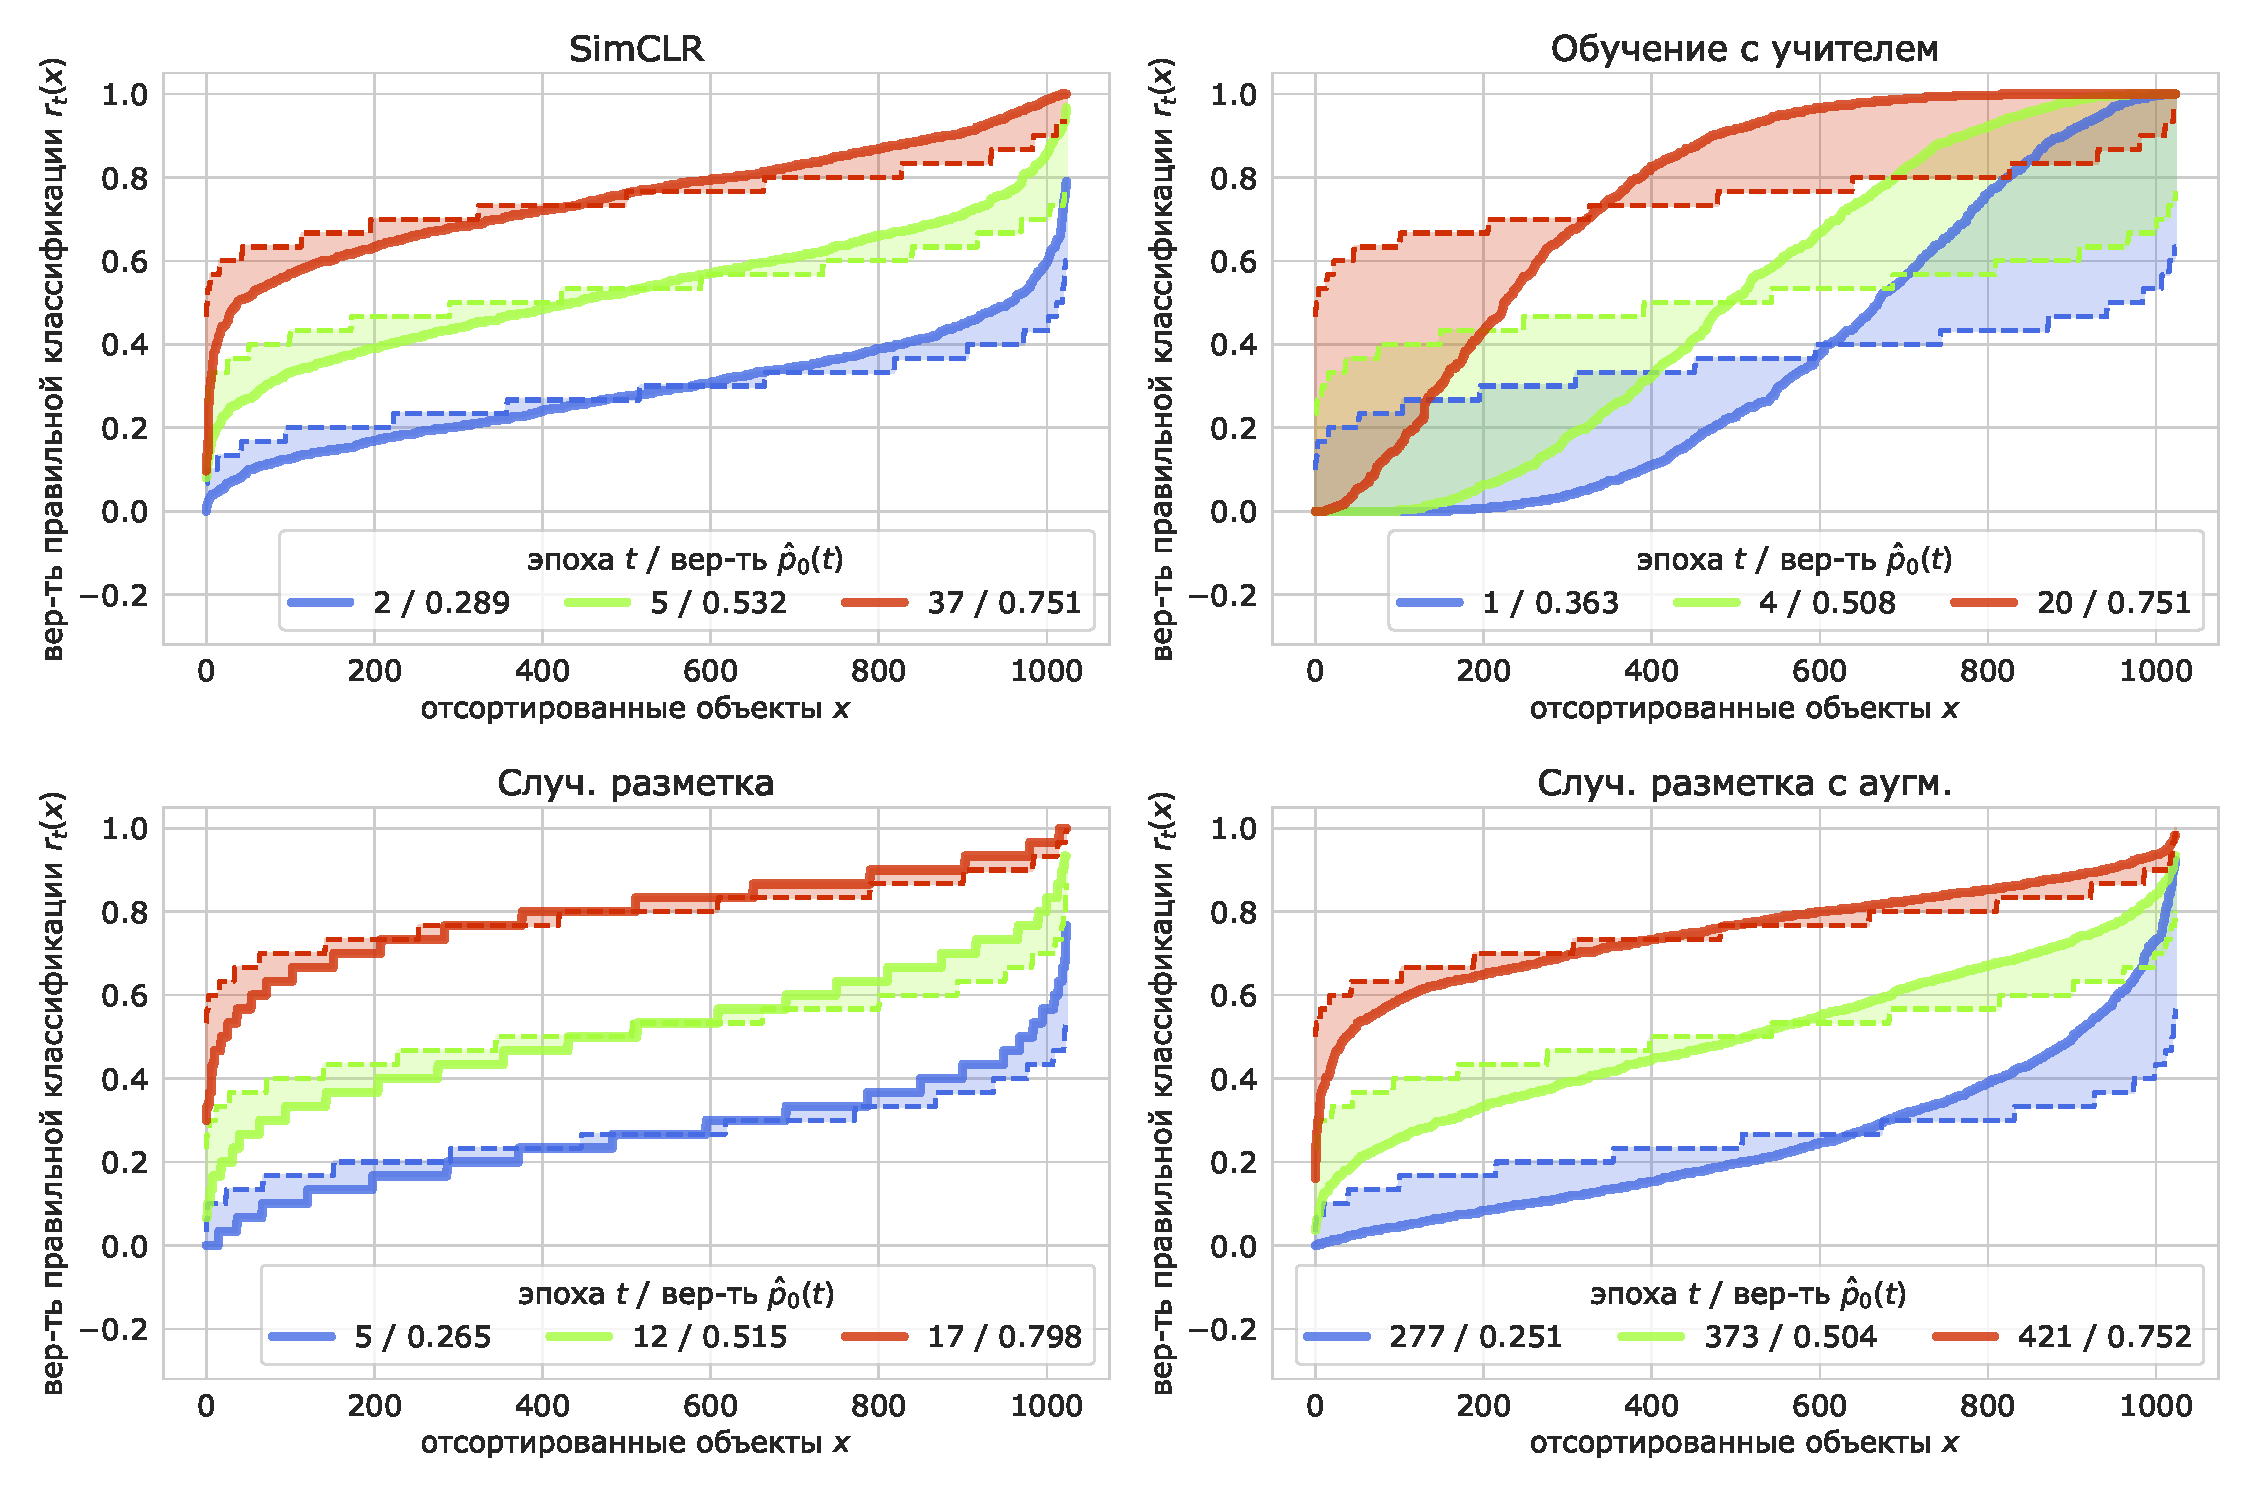
\includegraphics[width=17cm]{images/binom_noise2.pdf}
    \caption{Сравнение величины $r_t(x)$ (сплошная жирная линия) с соответствующим биномиальным шумом (пунктирная линия).}
    \label{experiments:pic:4}
\end{figure}{}

На рис. \ref{experiments:pic:4} и в таблице \ref{experiments:table:2} показаны результаты сравнения величины $r_t(x)$ с биномиальным шумом. Данный эксперимент подтверждает, что метод SimCLR и обе вариации обучения со случайной разметкой имеют меньший разброс сложностей объектов, чем обучение с учителем. Сравнивая данную группу графиков с предыдущей, мы приходим к выводу, что усреднение по аугментациям выравнивает сложности объектов в методе SimCLR. Заключительный эксперимент текущей серии проверяет данную гипотезу.

\begin{table}[H]
    \centering
    \begin{tabular}{|C{2.5cm}|C{1.75cm}|C{2.75cm}|C{3.25cm}|}
        \hline
        Метод & Эпоха $t$ & Вер-ть $\widehat{p}_0(t)$ & МАЕ ($\mu \pm \sigma$) \\ \hline
        \multirow{3}{*}{SimCLR} & 2 & 0.289 & $0.042 \pm 0.001$ \\ \cline{2-4}
        & 5 & 0.532 & $0.055 \pm 0.002$ \\ \cline{2-4}
        & 37 & 0.751 & $0.048 \pm 0.001$ \\ \hline
        \multirow{3}{*}{\shortstack{Обучение \\ с учителем}} & 1 & 0.363 & $0.248 \pm 0.001$ \\ \cline{2-4}
        & 4 & 0.508 & $0.267 \pm 0.002$ \\ \cline{2-4}
        & 20 & 0.751 & $0.208 \pm 0.001$ \\ \hline
        \multirow{3}{*}{\shortstack{Случ. \\ разметка}} & 5 & 0.265 & $0.037 \pm 0.002$ \\ \cline{2-4}
        & 12 & 0.515 & $0.052 \pm 0.001$ \\ \cline{2-4}
        & 17 & 0.798 & $0.031 \pm 0.002$ \\ \hline
        \multirow{3}{*}{\shortstack{Случ. \\ разметка \\ с аугм.}} & 277 & 0.251 & $0.093 \pm 0.002$ \\ \cline{2-4}
        & 373 & 0.504 & $0.081 \pm 0.001$ \\ \cline{2-4}
        & 421 & 0.752 & $0.038 \pm 0.002$ \\ \hline
    \end{tabular}
    \caption{Результаты сравнения величины $r_t(x)$ с биномиальным шумом. Для каждого подсчета метрики MAE было сгенерировано по 10 выборок биномиального шума, в таблице представлены среднее значение и стандартное отклонение.}
    \label{experiments:table:2}
\end{table}

На рис. \ref{experiments:pic:5} показано, как именно распределена величина $\tilde{r}_t(\tilde{x})$ для каждого фиксированного объекта $x$ и его аугментаций $\tilde{x} \sim \mathcal{A}(\tilde{x}|x)$. Согласно графику, в методе SimCLR многие аугментированные версии изображений являются либо очень сложными, и почти никогда не классифицируются правильно, либо очень простыми, и почти всегда верно распознаются нейронной сетью. Тем не менее, сами объекты тоже обладают разной сложностью: некоторые из них в принципе не имеют простых (или сложных) аугментаций. Напротив, при обучении с учителем и со случайной разметкой сложность аугментаций отличается не сильно: точки для разных аугментаций расположены вблизи среднего значения.

Мы связываем данный эффект с тем, что метод SimCLR использует более интенсивные аугментации. Они необходимы, чтобы сделать задачу разбиения изображений на пары достаточно сложной. Решение подобной задачи заставляет нейронную сеть выделять семантические закономерности изображений, что будет показано в \hyperref[visual:1]{разделе 5.1}.

\begin{figure}[H]
    \centering
    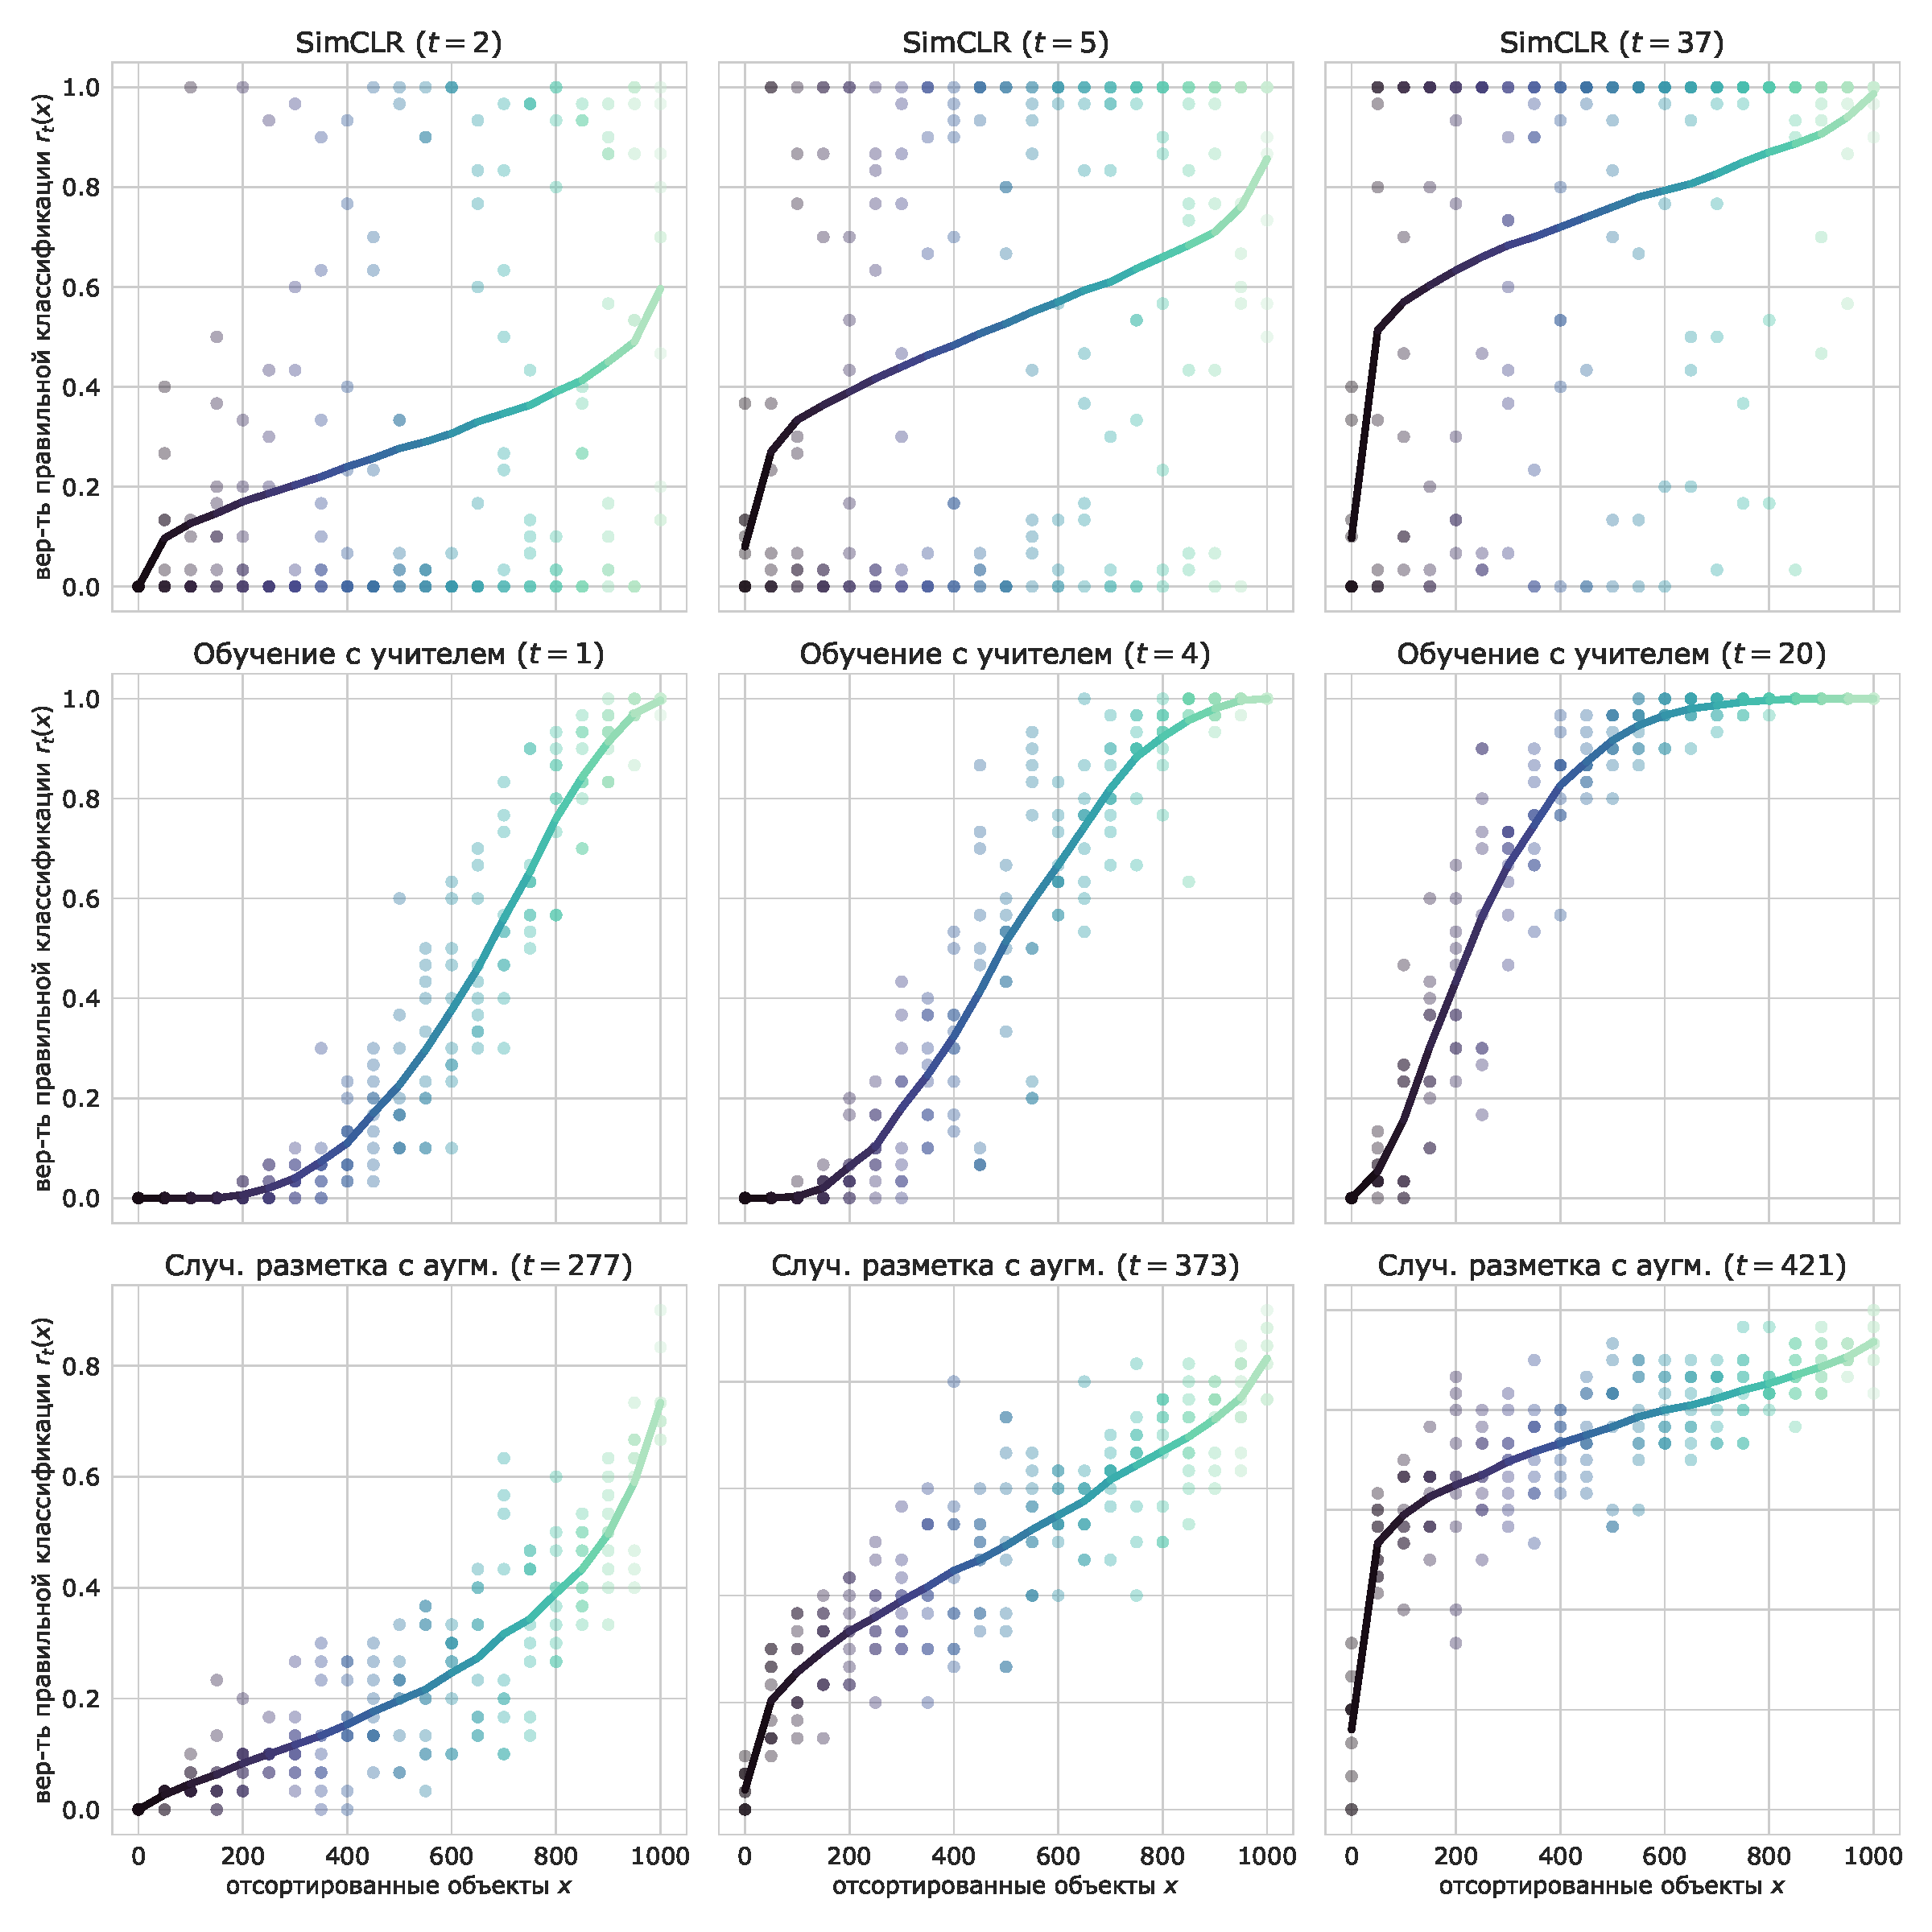
\includegraphics[width=17cm]{images/augments.pdf}
    \caption{Влияние аугментаций на сложности объектов для методов обучения. Каждая точка на графике --- значение $\tilde{r}_t(\tilde{x})$ для одной аугментации $\tilde{x}$. Для отображения был выбран каждый 50-ый объект среди отсортированной обучающей подвыборки. Сплошная кривая представляет собой усреднение по аугментациям, то есть величину $r_t(x)$.}
    \label{experiments:pic:5}
\end{figure}{}

Итак, эксперименты данного раздела демонстрируют, что для каждого алгоритма обучения существуют априорные сложности объектов: какие-то изображения распознаются нейронной сетью лучше и чаще классифицируются правильно; на других изображениях, напротив, нейронная сеть чаще ошибается. При этом описанный эффект в большей или меньшей степени проявляется для всех алгоритмов. Мы констатируем, что наибольший разброс сложности объектов наблюдается при обучении с учителем. Также мы показываем, что аугментации в методе SimCLR приводят к дополнительному ''расслоению'' сложностей: если зафиксировать по одной аугментации изображения, то разброс сложностей напоминает обучение с учителем. Однако усреднение по аугментациям выравнивает сложности объектов, и по данному показателю метод SimCLR становится похож на обучение со случайной разметкой.
